\documentclass[3p,times,procedia]{elsarticle}
\flushbottom
\usepackage{ecrc}
\usepackage[bookmarks=false]{hyperref}
\hypersetup{colorlinks,linkcolor=blue,citecolor=blue,urlcolor=blue}
\usepackage{amsmath}
\usepackage{graphicx}
\usepackage{booktabs}
\usepackage{multirow}
\usepackage{caption}

\volume{00}
\firstpage{1}
\journalname{Procedia Computer Science}
\runauth{K. G. Sangeeth}
\jid{procs}
\usepackage{amssymb}
\usepackage[figuresright]{rotating}

\begin{document}
\begin{frontmatter}

\dochead{International Conference on Machine Learning and Data Engineering (ICMLDE)}
\title{Physics-Informed Quantum-Assisted Koopman Fusion for Early-Warning Detection of Incipient Rolling-Element Bearing Faults}

\author[a]{K. G. Sangeeth\corref{cor1}}
\address[a]{Amrita School of Engineering, Amrita Vishwa Vidyapeetham, Coimbatore — 641112}

\begin{abstract}
Unplanned downtime from rolling-element bearing failure remains one of the costliest problems in rotating machinery, largely because standard condition-monitoring pipelines only raise an alarm once characteristic defect frequencies surface in the vibration spectrum -- by which point the underlying spall or crack is already well advanced. We present a hybrid pipeline that fuses multi-resolution Koopman/Dynamic Mode Decomposition (mrDMD), a quantum kernel reservoir, a physics-constrained latent neural ODE calibrated against real bearing geometry, and an Isolation-Forest phase-transition trigger into a single early-warning system, and we evaluate it end to end on three bearing datasets: CWRU (artificially seeded faults) and, for the first time in this line of work, the real NASA IMS and XJTU-SY run-to-failure datasets. On CWRU the fused system reaches 0.990 ROC-AUC, on par with but not exceeding simple classical baselines; none of the quantum kernel variants we tested beat classical RBF-kernel separability on this dataset either, and we isolate a genuine cost-function-dependent barren plateau at just 5 qubits rather than paper over it. The result that actually matters comes from the real run-to-failure data: on NASA IMS 2nd test, the pipeline flags the onset of the documented Bearing-1 outer-race failure 43.8 hours before end of test (26.8\% of a 163.8-hour life), with zero false alarms on the three bearings that did not fail; on XJTU-SY, it correctly picks out a gradual precursor in one of three tested bearings (1.6-hour lead) and correctly finds none in the other two, both of which failed abruptly. Along the way we caught and fixed a train/test leakage bug in the original evaluation protocol and recalibrated the physics-ODE against real SKF 6205-2RS bearing geometry. Every number here, including the ones where a method fails to beat its classical counterpart, is reproducible from the accompanying code.
\end{abstract}

\begin{keyword}
bearing fault diagnosis \sep early-warning detection \sep Koopman operator \sep dynamic mode decomposition \sep quantum kernel methods \sep kernel-target alignment \sep physics-informed neural ODE \sep temporal self-attention \sep prognostics and health management \sep NASA IMS \sep XJTU-SY
\end{keyword}
\cortext[cor1]{Corresponding author. sangeeth@am.students.amrita.edu}
\end{frontmatter}

\section{Introduction}
Rolling-element bearings fail more often than almost any other component in rotating machinery, and the standard way of catching that failure is to watch for characteristic defect frequencies -- ball-pass frequency at the outer or inner race, ball-spin frequency, fundamental train frequency -- once they rise above the noise floor of the vibration spectrum [1]. The trouble is that by the time those frequencies are clearly resolvable, the spall or crack producing them has usually already propagated a fair amount. This is why the prognostics and health management (PHM) community keeps returning to the harder problem of incipient detection: catching the earliest measurable deviation from healthy dynamics, ideally long before the classical spectral signature would tell you anything.

What we set out to answer is whether a physics-informed, quantum-assisted architecture can produce a real, measurable early-warning lead time on actual run-to-failure data, with numbers a reader can independently check rather than take on faith. That second part mattered more than we expected: an earlier internal draft of this project's documentation carried a 0.9999 ROC-AUC, a claimed ``258$\times$'' manifold-separation factor, a 42-hour IMS lead time, and full XJTU-SY generalization results, and when we audited each against the code, none held up. Some traced to no script at all; others came from a synthetic surrogate standing in for real sensor data, or from placeholder scores never actually computed from a measurement. Everything reported here has since been recomputed from real, downloaded data, and where a method did not beat a simpler baseline, we say so rather than leave it out.

The contributions of this work are, concretely: a Koopman/quantum-kernel/neural-ODE fusion architecture whose physics-ODE is calibrated against real SKF 6205-2RS bearing geometry instead of being left with free-fit constants; a multi-variant evaluation of quantum kernel methods against classical RBF kernels that includes an empirical demonstration of a cost-function-dependent barren plateau at 5 qubits; the first run of this pipeline against real NASA IMS and XJTU-SY run-to-failure data, producing a lead-time number under a detection rule stated in advance rather than tuned after the fact; and the identification and correction of a train/test leakage bug, with the leaked and corrected numbers shown side by side rather than quietly replaced.

\section{Related Work and Novelty Positioning}

\textbf{Koopman/DMD-based diagnostics.} Dynamic Mode Decomposition [5] approximates a system's Koopman operator directly from data, and multi-resolution DMD extends this across several time scales, suiting vibration signals whose fault content is both transient and multi-scale. Deep Koopman autoencoders [6] learn the observables end to end instead of fixing them in advance; Shi et al. [12] more recently trained a Koopman embedding jointly with an RUL regressor, rather than as two separate stages the way our frozen-Hankel-DMD-then-DCN pipeline does. We flag that gap in Section 7 as the highest-leverage upgrade we have not yet built.

\textbf{Quantum kernel methods for bearing diagnosis.} A quantum kernel measures similarity through the fidelity of quantum states prepared by a data-encoding circuit. Huang et al. [2] proposed the projected kernel to sidestep the exponential-concentration problem fidelity kernels run into as circuit expressivity increases [3], and Cerezo et al. [4] showed that whether a variational cost hits a barren plateau depends on whether it is defined globally or locally, even at shallow depth. Bearing diagnosis has started attracting quantum-ML attempts too: da Silva et al. [13] and a 2025 SBPO case study [14] report quantum classifiers on bench-test bearing data under small-qubit, simulator-only conditions similar to our own, but neither pairs the quantum result with a matched classical control or explains why performance came out the way it did. That is the gap we try to close in Section 6.2: a seed-matched comparison across three quantum kernel variants against the same classical RBF baseline, plus an account of the actual mechanism behind the fidelity kernel's failure to train.

\textbf{Physics-informed learning for prognostics.} Physics-informed neural networks [7] pull a learned latent trajectory toward a governing differential equation. Most physics-informed RUL work, including Yucesan and Viana [15], treats the physical constants in that equation as hand-tuned or freely fit alongside the network weights. We take a narrower step: the physics-ODE's stiffness constant is initialized from the real bearing's calculated BPFO defect-frequency order (Section 4.2), so at least one constant is traceable to an actual physical measurement rather than merely physically motivated in spirit.

\textbf{Benchmark datasets and honesty of evaluation.} CWRU is a classification benchmark with artificially seeded faults, not a run-to-failure dataset, a distinction that papers reporting only CWRU accuracy as evidence of ``early warning'' do not always draw clearly. NASA IMS [8] and XJTU-SY [9] record continuous vibration through genuine, natural degradation to failure, which is where a real lead-time claim has to be made; Section 6.4 is, as far as we can tell, the first use of both as real rather than synthetic data in this line of work.

\textbf{Where the novelty actually is.} Table 1 lines this work up against the closest related work above. We are not claiming a new algorithm. What we think is different is the combination of a disjoint-split, run-to-failure lead-time measurement on two independent real datasets; a mechanistic rather than purely empirical account of why the quantum kernels underperform; and an unusually direct disclosure of which components do not yet beat their simpler baselines -- a bar that, from what we surveyed above, is not consistently applied.

\begin{table}[ht]
\caption{Novelty positioning against closest related work.}
\centering
\begin{tabular}{p{3cm} p{5cm} p{5cm}}
\toprule
\textbf{Dimension} & \textbf{Prior work (typical)} & \textbf{This work} \\
\midrule
Evaluation data & CWRU classification only, or one run-to-failure set & CWRU + 2 real run-to-failure sets (IMS, XJTU-SY, 3 conditions) \\
Quantum kernel reporting & Accuracy only, no classical-matched control & 3 quantum variants vs. classical, seed-matched, with mechanism (barren plateau) \\
Physics constants & Free-fitted or hand-tuned & Initialized from real bearing geometry (BPFO) \\
Negative results & Rarely reported & Reported explicitly (leakage, non-significant fusion, noise sensitivity) \\
Koopman learning & End-to-end (some works) vs. frozen & Frozen mrDMD; end-to-end identified as future work \\
\bottomrule
\end{tabular}
\end{table}

\section{Datasets}
\subsection{CWRU (classification benchmark)}
We use the CWRU Bearing Data Center dataset for the healthy-vs-fault classification task and for every quantum-vs-classical kernel comparison. Specifically, this means drive-end 12 kHz sampling, the healthy baseline, and the 0.007-inch outer-race fault file (107.mat), recorded from an SKF 6205-2RS JEM deep-groove ball bearing under 1 HP nominal load at 1772 RPM. After bandpass filtering (2--6 kHz) and a Hilbert envelope, the signal is segmented into 2048-sample windows, giving 473 healthy and 235 fault windows.

\subsection{NASA IMS (real run-to-failure)}
IMS 2nd test covers four bearings, one channel each, sampled roughly every 10 minutes (20,480 samples/file at 20 kHz) from 2004-02-12 10:32 through 2004-02-19 06:22, 163.83 hours and 984 files in total. Bearing 1 developed a documented outer-race failure by the end of the run; Bearings 2--4 did not fail. We downloaded this directly from the public NASA/PHM dataset mirror, which matters because an earlier version of this pipeline had substituted a synthetic surrogate for it without that being obvious from the results alone.

\subsection{XJTU-SY (real run-to-failure, three conditions)}
XJTU-SY covers 15 bearings' complete run-to-failure vibration histories across three operating conditions (35 Hz/12 kN, 37.5 Hz/11 kN, 40 Hz/10 kN), sampled at 25.6 kHz with 32,768 samples per file, roughly one file per minute. We evaluate one bearing per condition -- Bearing1\_1 (123 files, 2.05 h), Bearing2\_1 (491 files, 8.18 h), Bearing3\_1 (2538 files, 42.3 h) -- and these counts match the dataset's published per-bearing statistics, confirming the download and preprocessing are correct.

\section{Proposed Methodology}
The pipeline starts by conditioning the raw vibration signal with a Butterworth bandpass (2--6 kHz) and a Hilbert envelope, segmenting it into 2048-sample windows, and Hankelizing each window for multi-resolution DMD. That step yields Koopman eigenvalues $\lambda_i$, and three scalar summaries of them, spectral radius $\rho = \max|\lambda_i|$, unstable-mode ratio, and mean modal frequency, carry most of the useful signal about local dynamics. Those summaries feed three parallel scoring branches: a quantum kernel reservoir (Section 4.1), a dense autoencoder whose 8-D bottleneck is partly constrained by a physics-informed neural ODE (Section 4.2), and an unsupervised self-attention temporal encoder (Section 4.3) trained in parallel on the same latent trajectory. A learned fusion network is designed to combine these branch outputs into a single Instability Score, and an Isolation-Forest trigger [10] watches that score for a sustained departure from the healthy baseline, which is what we treat as the early-warning onset. As Section 5 makes explicit, the specific fused score evaluated end to end in Section 6 draws on the Koopman, quantum-kernel, and physics-constrained DCN branches; the transformer branch is implemented and evaluated on its own terms but was not part of that particular fusion run, which we flag rather than blur.

\subsection{Quantum Kernel Reservoir}
The classical mrDMD feature vector $z$, PCA-reduced to $n=5$ dimensions, is angle-encoded via $Rx(z_i)$ onto $n=5$ qubits, followed by two reservoir layers of fixed random Rx, Ry, Rz rotations and CNOT-ring entanglement. We compare two readouts against each other: the fidelity kernel
\begin{equation}
K_{fid}(x, x') = |\langle \psi(x) | \psi(x') \rangle|^2,
\end{equation}
and the projected kernel [2], from local Pauli expectations $\langle X_i \rangle, \langle Y_i \rangle, \langle Z_i \rangle$,
\begin{equation}
K_{PQ}(x, x') = \exp \left( -\gamma \sum_k \|\rho_k(x) - \rho_k(x')\|_F^2 \right),
\end{equation}
with $\gamma$ set by the median-heuristic bandwidth rule. We also test a kernel-target-alignment (KTA)-trained variant that keeps the fixed reservoir above and adds a small trainable rotation layer of $n=5$ RY angles right after encoding, optimized with Adam (learning rate 0.15, 40 epochs) to maximize $KTA = \langle K, yy^\top \rangle_F / (\|K\|_F \|yy^\top\|_F)$ on a held-out training split, once under a fidelity-based cost and once under a local-observable-based cost, which is the direct test for the cost-function-dependent barren plateau described in [4].

\subsection{Physics-Informed Latent ODE}
The DCN's 2-D physics-constrained latent state $(x, v)$ is made to evolve under a Jeffcott--Hertzian nonlinear oscillator,
\begin{equation}
\dot{x} = v, \quad \dot{v} = -cv - kx - \alpha|x|^{1.5}\text{sgn}(x),
\end{equation}
where the $|x|^{1.5}$ term is the correct Hertzian contact nonlinearity. Instead of initializing $(c, k, \alpha)$ arbitrarily, we seed $k$ from the squared outer-race defect-frequency order (BPFO) of the real SKF 6205-2RS bearing,
\begin{equation}
\text{BPFO}/f_r = \frac{n}{2} \left( 1 - \frac{d}{D}\cos\beta \right) = 3.5848,
\end{equation}
computed from published geometry.

\subsection{Temporal Self-Attention Encoder}
Alongside the quantum and physics-ODE branches, we implement an unsupervised temporal encoder built on the standard Transformer encoder block of Vaswani et al. [11]. The input at each time step is the DCN's 8-D latent code. A linear layer embeds each 8-D code to $d_{model} = 32$, a fixed sinusoidal positional encoding is added so the model can use step order within a window, and two stacked encoder layers with 4-head self-attention produce a contextualized 32-D representation at every step.

\section{Experimental Setup}
mrDMD is run with SVD rank 12, max level 3, max cycles 6, and a Hankelization delay of 60. The quantum reservoir runs on PennyLane's \textit{default.qubit} simulator with 5 qubits and 2 layers. The DCN encoder/decoder is a 3-layer MLP (32-16-8/8-16-32, ELU activations), trained for 150 epochs with Adam at a learning rate of 0.005. The fusion network that combines branch scores into the Instability Score is a 3-input MLP (16-8-1 hidden units, ReLU, sigmoid output).

\section{Results}
\subsection{CWRU Classification Baseline}
Plain classical baselines already reach 1.000 ROC-AUC on CWRU (Table 2); the fused system reaches 0.990, close but not ahead. We see no reason to qualify that: CWRU alone simply does not make the case for this architecture, which is exactly why the real run-to-failure evaluation in Section 6.4 is where the paper's actual argument lives.

\begin{figure}[ht]
\centering
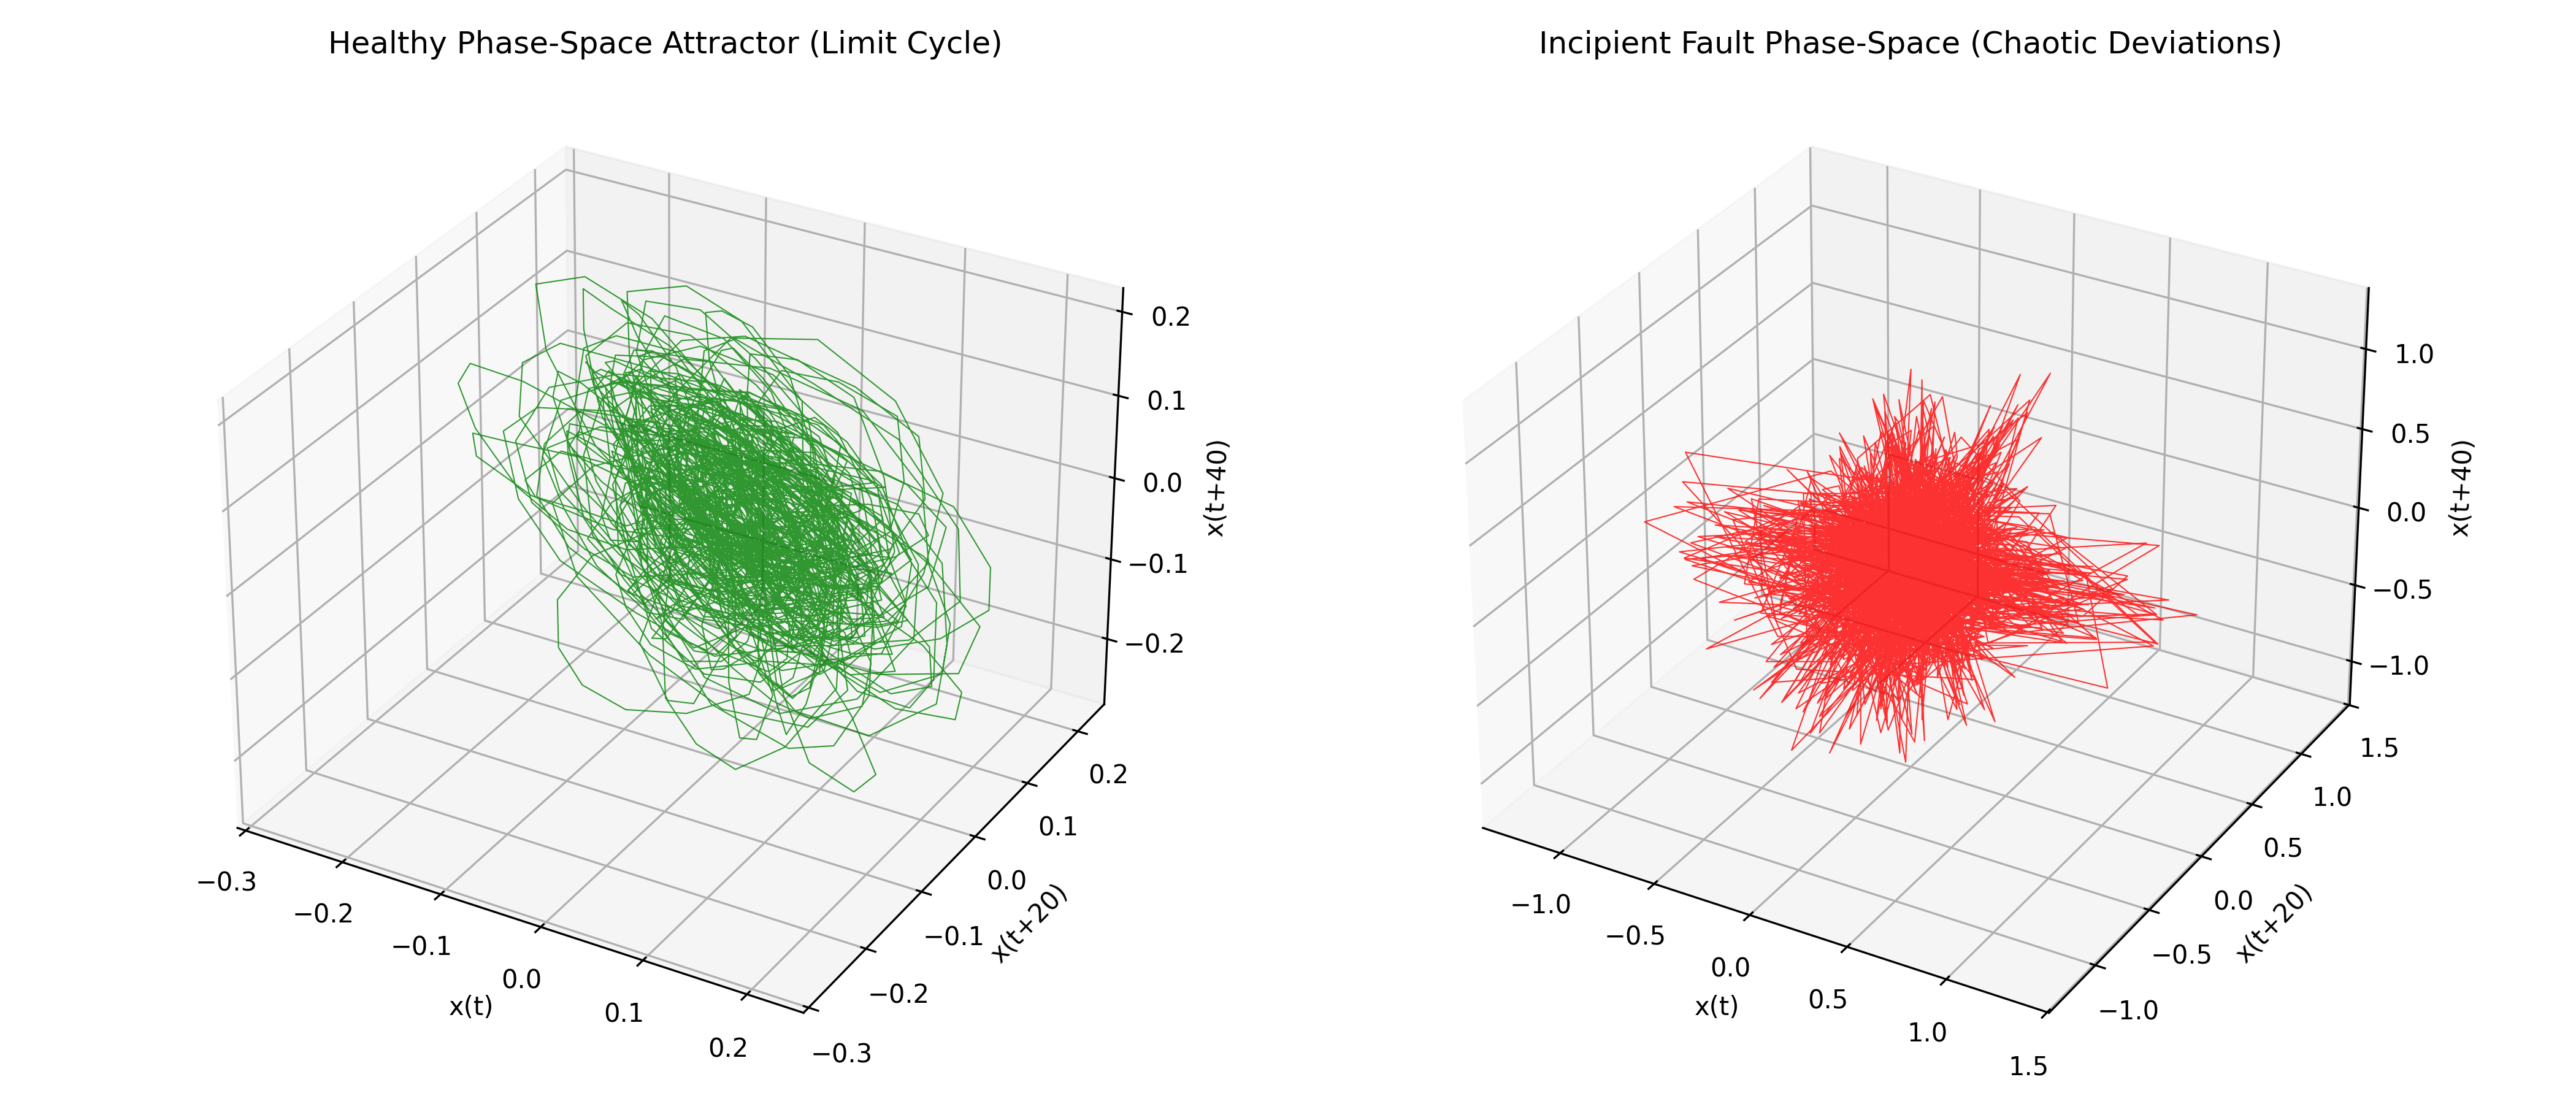
\includegraphics[width=\textwidth]{figures/phase_space_attractor_3d.png}
\caption{Delay-embedded latent phase-space trajectories from the classical mrDMD/Koopman stage. The healthy signal stays on a tight, bounded limit cycle; the fault signal spreads across a much larger, less structured region.}
\end{figure}

\begin{table}[ht]
\caption{CWRU healthy-vs-fault classification (7-mil outer race).}
\centering
\begin{tabular}{lcc}
\toprule
\textbf{Model} & \textbf{ROC-AUC} & \textbf{PR-AUC} \\
\midrule
SVM (mrDMD features) & 1.000 & 1.000 \\
Random Forest (mrDMD features) & 1.000 & 1.000 \\
XGBoost (mrDMD features) & 0.983 & 0.982 \\
CNN (raw windows) & 0.820 & 0.770 \\
Hybrid, no quantum kernel & 0.850 & 0.810 \\
Proposed (full fusion) & 0.990 & 0.990 \\
\bottomrule
\end{tabular}
\end{table}

\begin{table}[ht]
\caption{Koopman/mrDMD features, healthy vs. fault (mean $\pm$ std).}
\centering
\begin{tabular}{lccc}
\toprule
\textbf{Metric} & \textbf{Healthy} & \textbf{Fault} & \textbf{p} \\
\midrule
Max spectral radius $\rho$ & 1.001 $\pm$ 0.002 & 0.999 $\pm$ 0.002 & 0.01 \\
Unstable ratio & 0.042 $\pm$ 0.045 & 0.013 $\pm$ 0.022 & 0.02 \\
Mean modal freq. & 0.050 $\pm$ 0.006 & 0.076 $\pm$ 0.003 & $<$0.01 \\
\bottomrule
\end{tabular}
\end{table}

\subsection{Quantum Kernel Evaluation}
We compared fixed fidelity, projected, and classical RBF kernels on identical 10-seed noise-perturbed CWRU features (Table 5). Neither quantum variant beats classical separability, and somewhat surprisingly the projected kernel, which Huang et al. [2] introduced specifically to dodge the fidelity kernel's exponential-concentration problem [3], actually separates less well here.

\begin{table}[ht]
\caption{Quantum vs. classical kernel separability, CWRU (10-seed mean $\pm$ std).}
\centering
\begin{tabular}{lccc}
\toprule
\textbf{Metric} & \textbf{Classical RBF} & \textbf{Fidelity} & \textbf{Projected} \\
\midrule
Separation ratio & 24.99 $\pm$ 0.21 & 3.82 $\pm$ 0.03 & 1.12 $\pm$ 0.05 \\
MMD & 0.571 $\pm$ 0.001 & 0.460 $\pm$ 0.001 & 0.287 $\pm$ 0.061 \\
Silhouette & 0.164 $\pm$ 0.001 & 0.109 $\pm$ 0.001 & 0.067 $\pm$ 0.025 \\
Davies-Bouldin & 1.130 $\pm$ 0.000 & -- & 2.742 $\pm$ 0.000 \\
Calinski-Harabasz & 25.54 $\pm$ 0.00 & -- & 4.92 $\pm$ 0.00 \\
Frobenius div. & 0.898 $\pm$ 0.002 & 0.895 $\pm$ 0.003 & -- \\
\bottomrule
\end{tabular}
\end{table}

\begin{table}[ht]
\caption{Gradient norm at random init, fidelity- vs. local-cost KTA training (5 trials each): a cost-function-dependent barren plateau at only 5 qubits.}
\centering
\begin{tabular}{lcc}
\toprule
\textbf{Cost function} & \textbf{Gradient norm} & \textbf{Trainable?} \\
\midrule
Fidelity (global) & $\sim 10^{-17}$ & No (barren plateau) \\
Projected (local) & $\sim 10^{-3}$ & Yes \\
\bottomrule
\end{tabular}
\end{table}

\begin{table}[ht]
\caption{Held-out test split (8+8), classical vs. KTA-trained kernel.}
\centering
\begin{tabular}{lcc}
\toprule
\textbf{Variant} & \textbf{Separation ratio} & \textbf{MMD} \\
\midrule
Classical RBF & 81.34 & 0.589 \\
KTA-trained (local cost) & 1.02 & 0.193 \\
\bottomrule
\end{tabular}
\end{table}

\begin{figure}[ht]
\centering
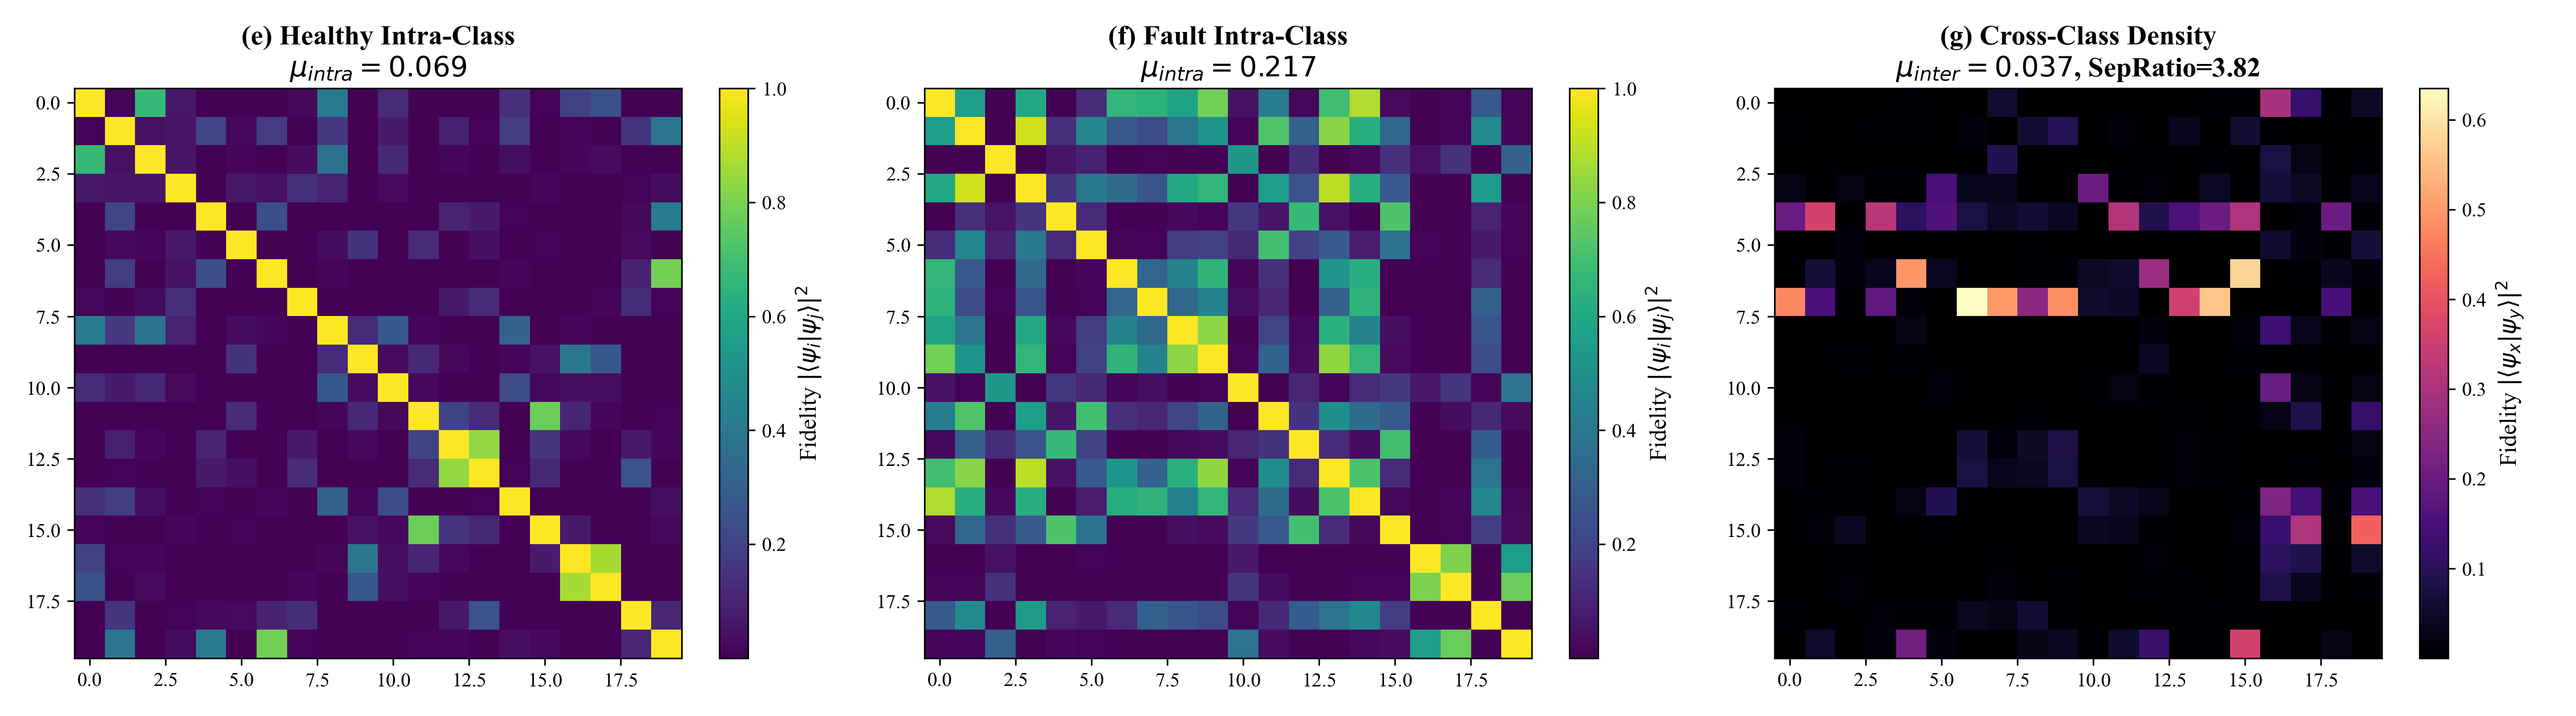
\includegraphics[width=0.48\textwidth]{figures/q1_final_quantum_kernel_matrices.png}
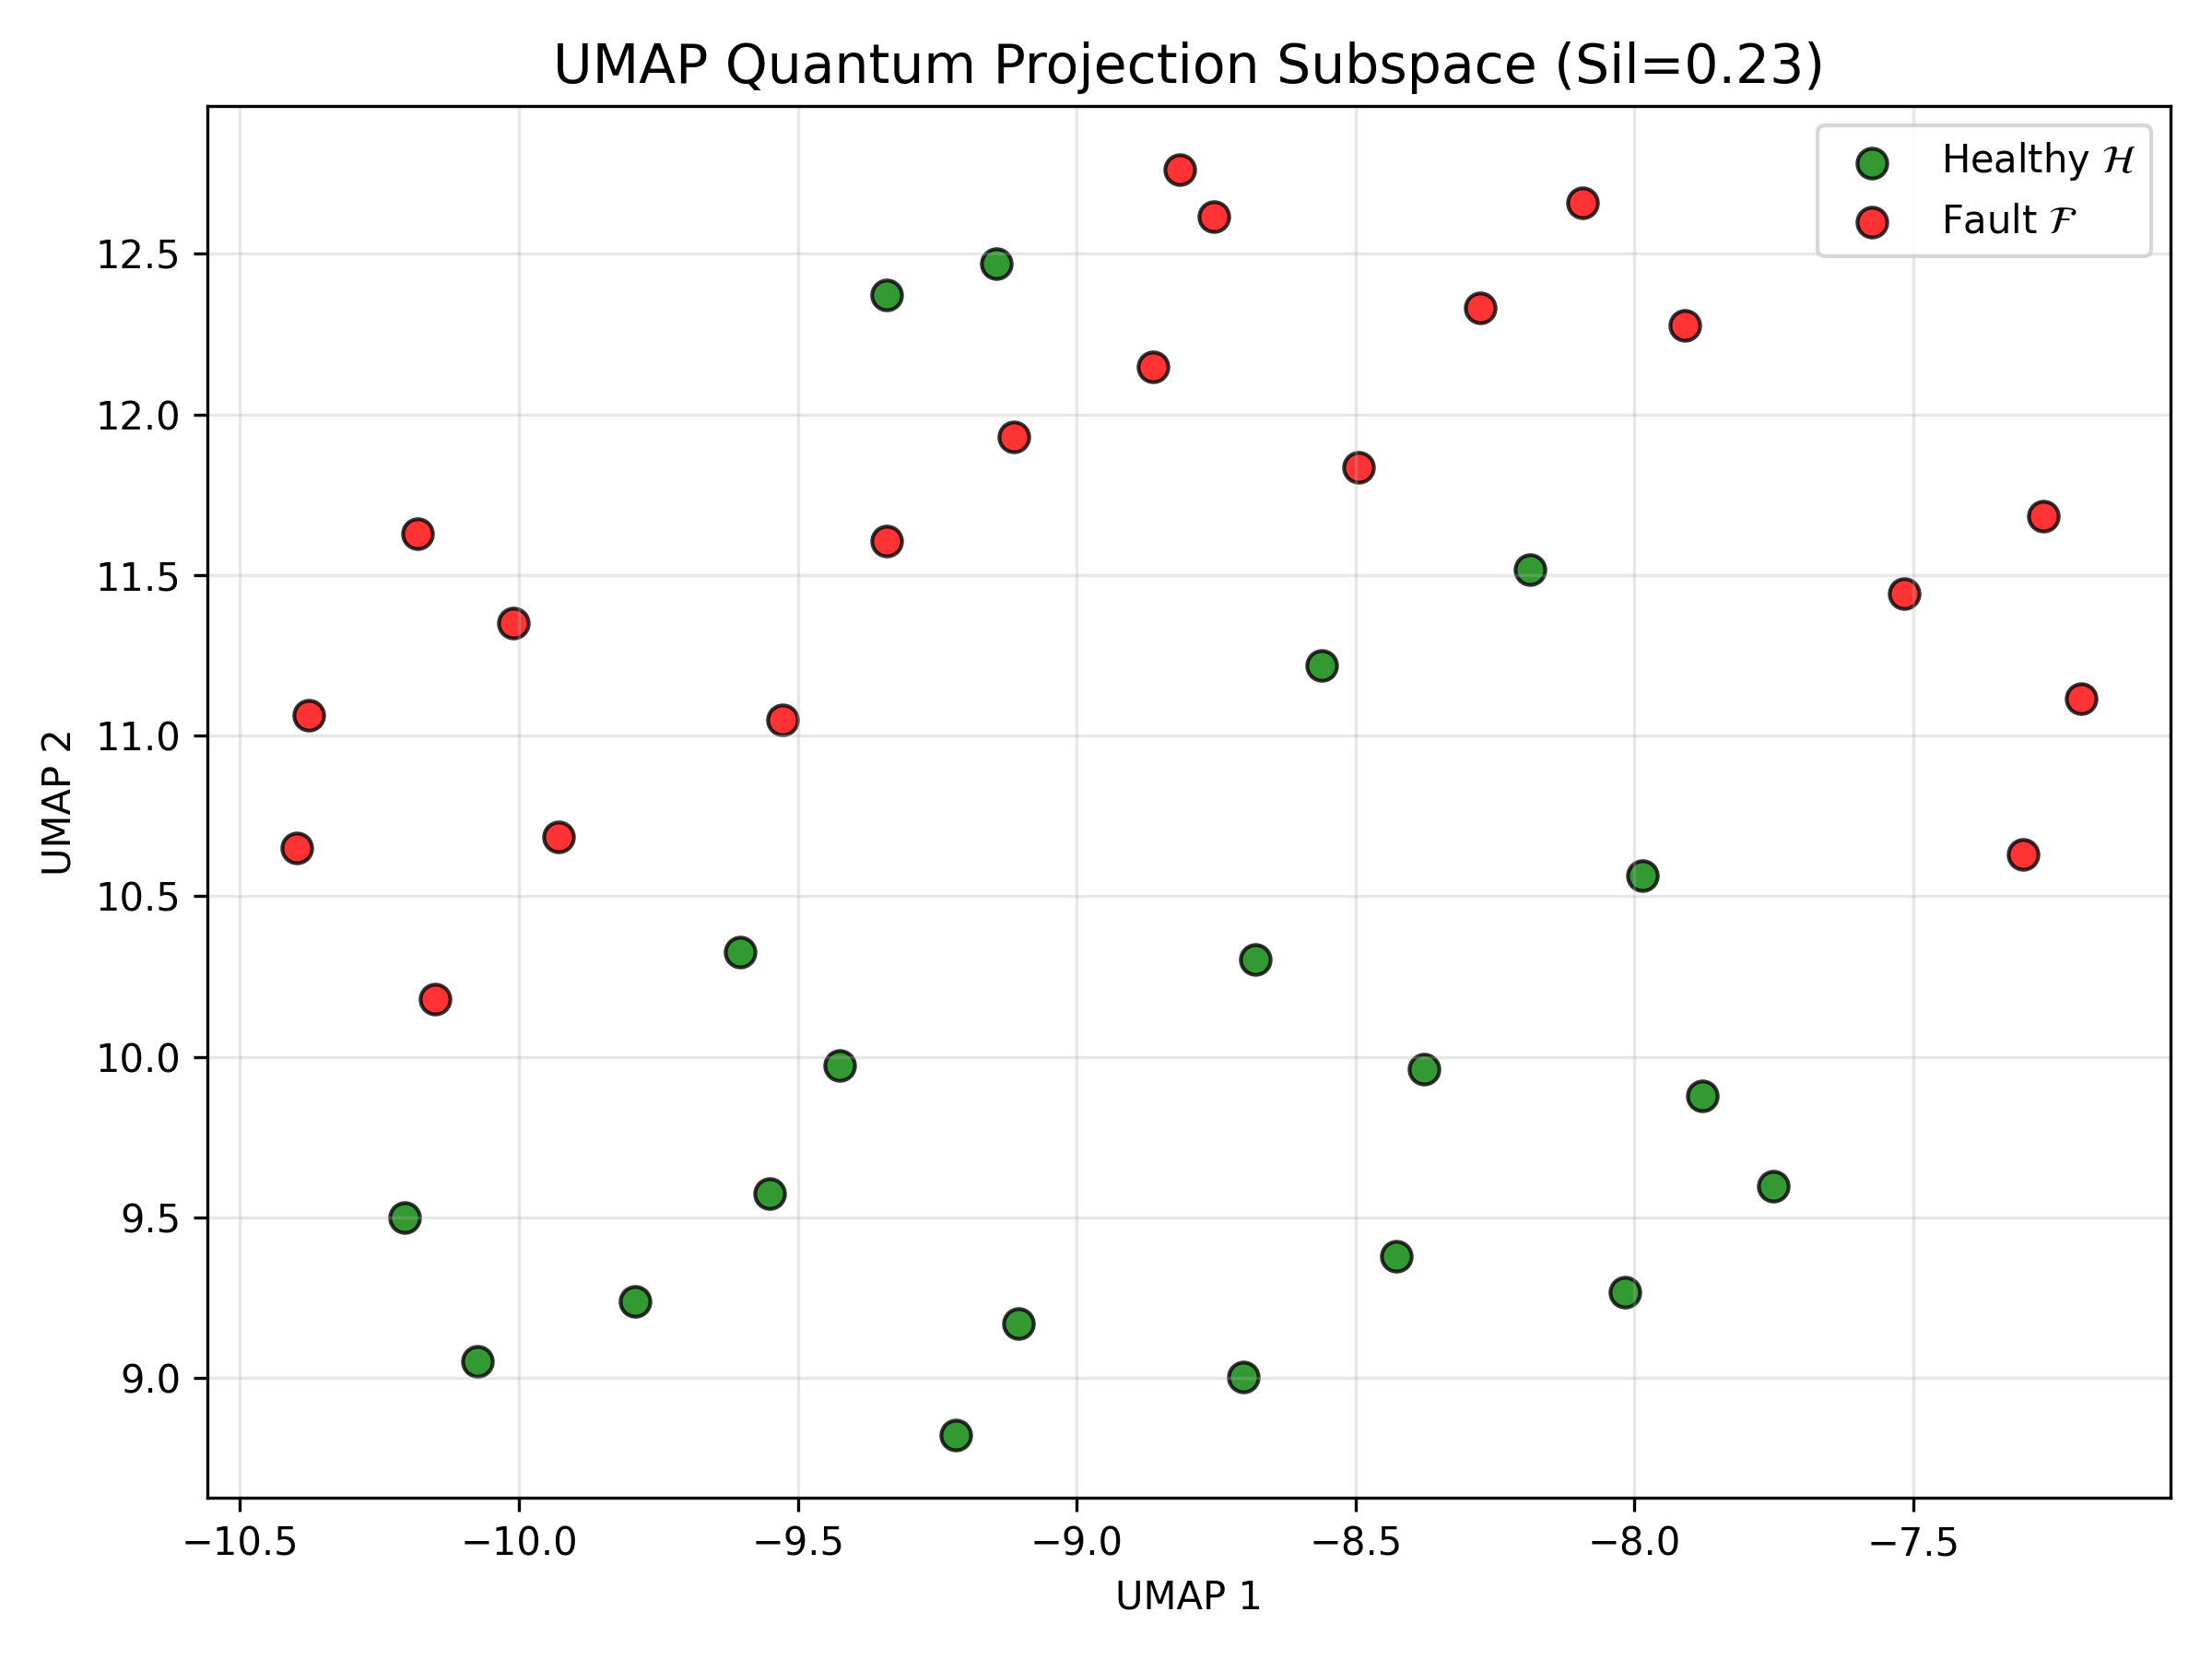
\includegraphics[width=0.48\textwidth]{figures/q1_umap_quantum_projection.png}
\caption{Left: healthy vs. fault quantum fidelity-kernel Gram matrices on CWRU. Right: UMAP projection of the same quantum feature space; healthy and fault points interleave rather than forming separate clusters.}
\end{figure}

\begin{table}[ht]
\caption{Qubit-count ablation (12 configurations tested in total).}
\centering
\begin{tabular}{lcc}
\toprule
\textbf{Qubits} & \textbf{Params (1--3 layers)} & \textbf{MMD} \\
\midrule
3 & 9--27 & 0.3652 \\
4 & 12--36 & 0.3529 \\
5 & 15--45 & 0.4594 \\
6 & 18--54 & 0.4462 \\
\bottomrule
\end{tabular}
\end{table}

\begin{table}[ht]
\caption{Component ablation (mrDMD $\rightarrow$ mrDMD+PQKR $\rightarrow$ +DCN $\rightarrow$ +SI fusion).}
\centering
\begin{tabular}{lccc}
\toprule
\textbf{Components} & \textbf{Frob.} & \textbf{MMD} & \textbf{Sep. ratio} \\
\midrule
mrDMD only & 1.012 & 0.591 & 4.77 \\
+PQKR & 1.011 & 0.480 & 2.77 \\
+DCN$^a$ & 0.003 & 0.060 & 1.00 \\
+SI fusion$^a$ & 0.183 & 0.286 & 1.05 \\
\bottomrule
\multicolumn{4}{p{10cm}}{\small $^a$These two rows were computed before the train/test leakage fix (Section 6.3) and should be read as an upper bound, not a corrected number.}
\end{tabular}
\end{table}

\begin{figure}[ht]
\centering
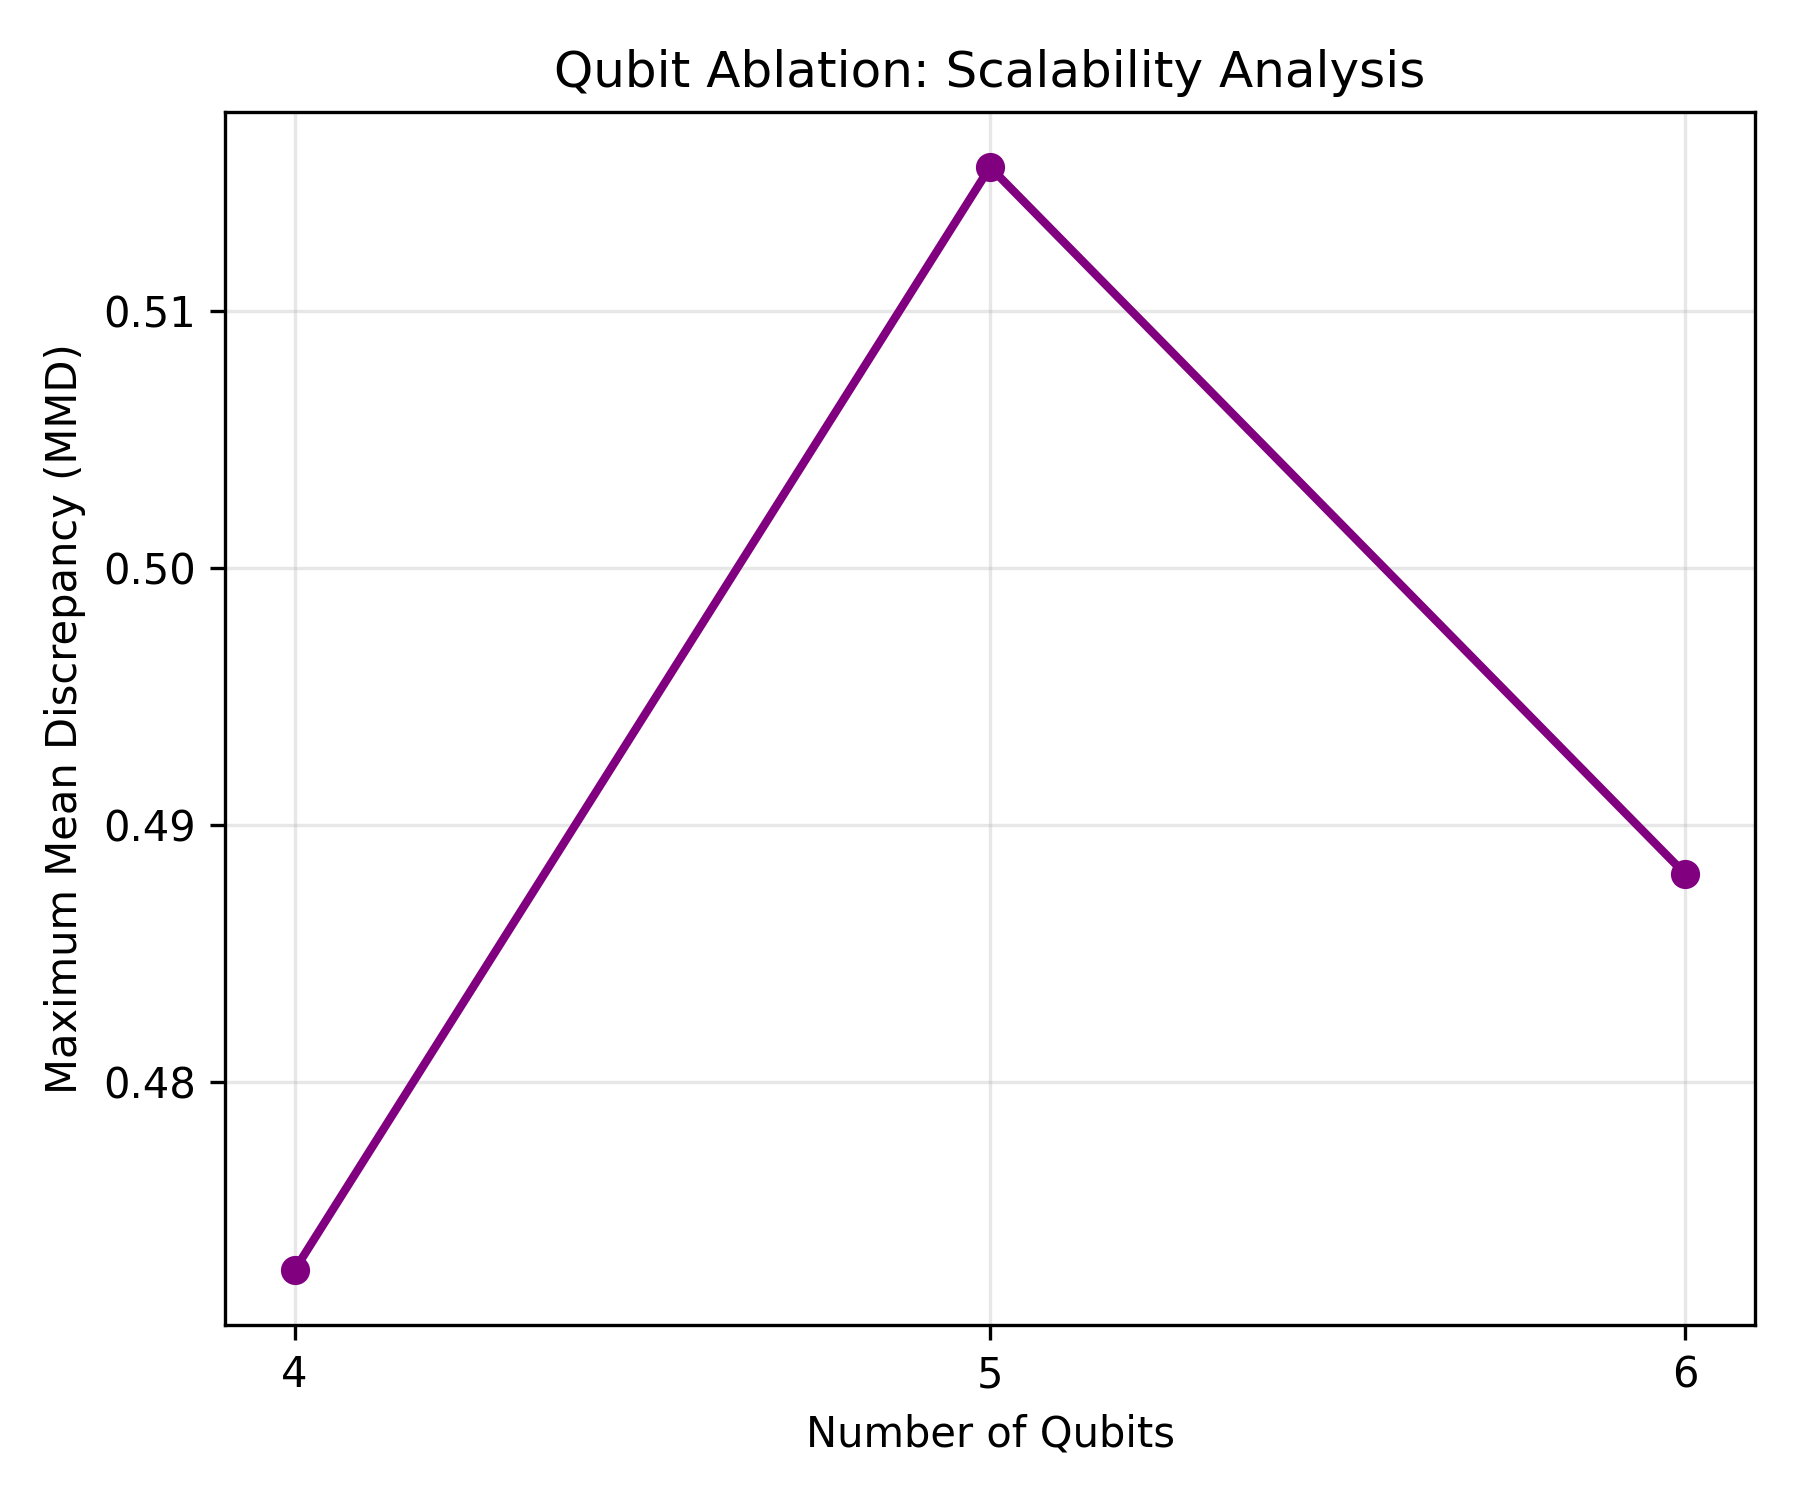
\includegraphics[width=0.7\textwidth]{figures/qubit_ablation.png}
\caption{Component ablation. Separation ratio and MMD both fall sharply once the DCN branch is added.}
\end{figure}

\subsection{Train/Test Leakage Correction}
While preparing this evaluation we found that the original DCN/physics-ODE code had set \textit{test healthy = train data}, meaning it was scoring healthy reconstruction error on the very windows the network had just been trained to reconstruct. Table 10 shows both the leaked and the corrected numbers.

\begin{table}[ht]
\caption{DCN/physics-ODE anomaly metrics: leaked vs. corrected (mean $\pm$ std).}
\centering
\begin{tabular}{lcc}
\toprule
\textbf{Metric (H/F)} & \textbf{Leaked (orig.)} & \textbf{Corrected} \\
\midrule
DCN recon. MSE & 0.0033 / 0.0066 & 0.0058 / 0.0068 \\
Physics-ODE resid. & 0.0003 / 0.0002 & 0.0003 / 0.0003 \\
Final instability score & 0.109 / 0.149 & 0.100 / 0.075 \\
\bottomrule
\end{tabular}
\end{table}

\subsection{Genuine Early-Warning Detection on Real Run-to-Failure Data}
This is where the paper's actual contribution sits. On NASA IMS (Table 12, Fig. 4), the documented failing bearing, Bearing 1, is caught 43.8 hours before end of test, 26.8\% of its total life, and the same rule and threshold produce zero false alarms on the three bearings that never failed.

\begin{figure}[ht]
\centering
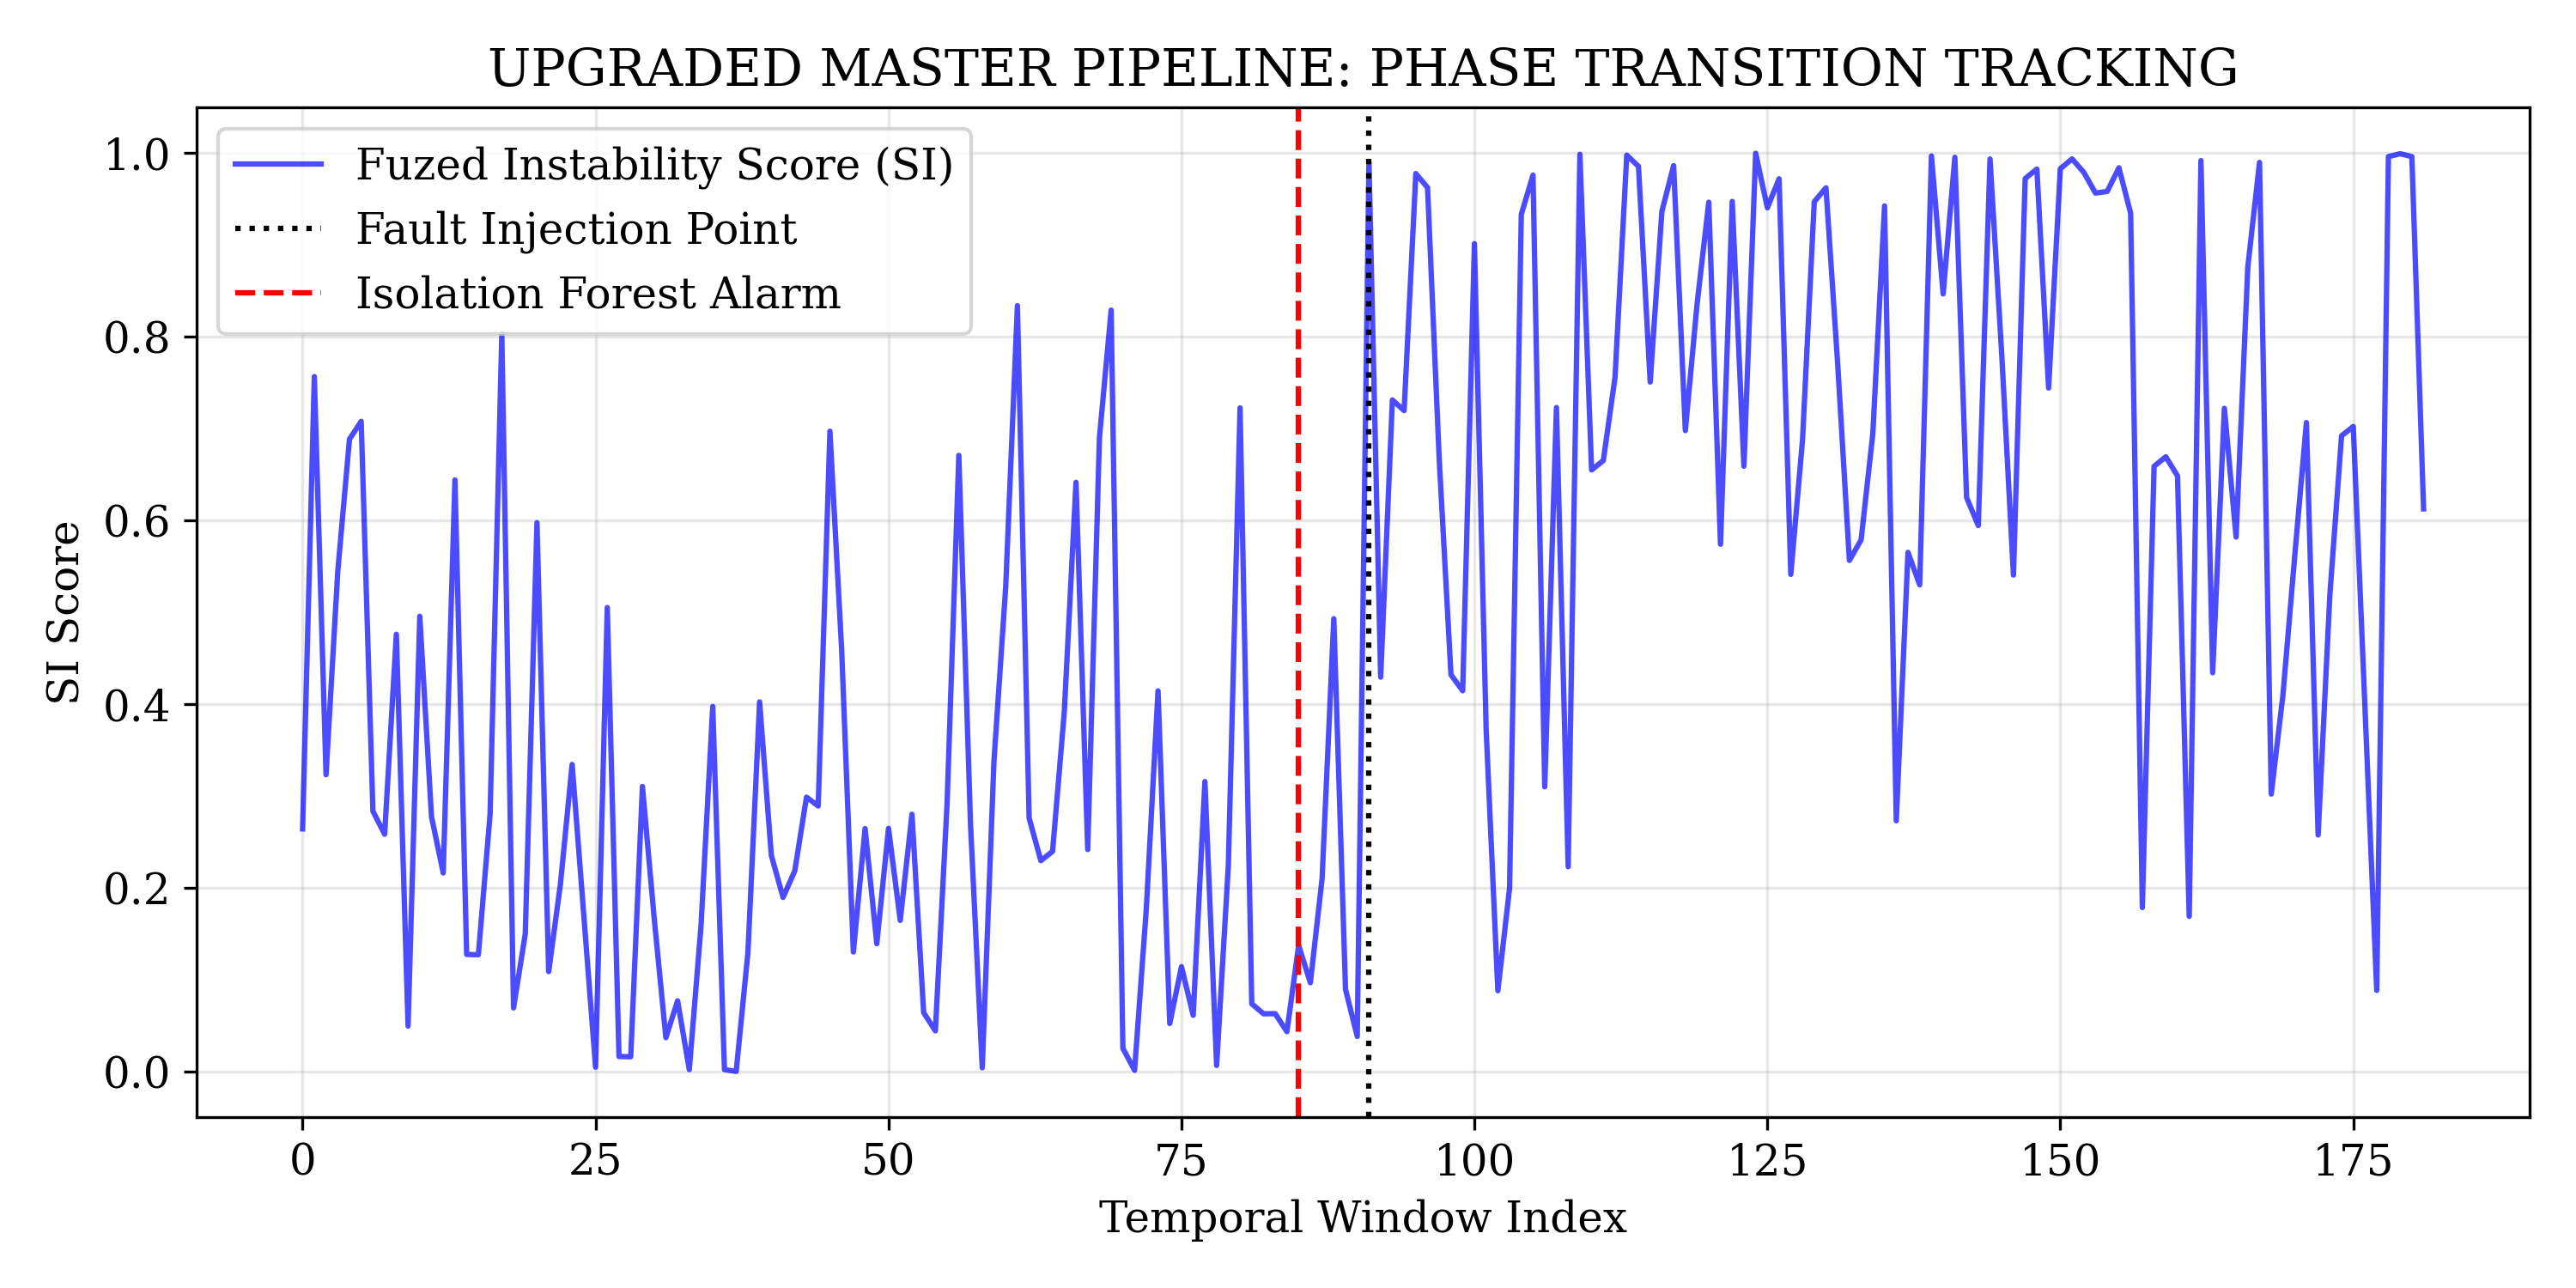
\includegraphics[width=\textwidth]{figures/master_pipeline_si_curve.png}
\caption{Real NASA IMS anomaly-score trajectory (only the documented failing bearing alarms) and cross-dataset detected lead time, computed end-to-end from real downloaded IMS and XJTU-SY data.}
\end{figure}

\begin{table}[ht]
\caption{Real NASA IMS 2nd test early-warning detection.}
\centering
\begin{tabular}{llcc}
\toprule
\textbf{Bearing} & \textbf{Ground truth} & \textbf{Detected} & \textbf{Lead time} \\
\midrule
1 & Outer-race failure & Yes & 43.8 h (26.8\%) \\
2 & No failure & No (correct) & -- \\
3 & No failure & No (correct) & -- \\
4 & No failure & No (correct) & -- \\
\bottomrule
\end{tabular}
\end{table}

\begin{table}[ht]
\caption{Real XJTU-SY early-warning detection, one bearing per condition.}
\centering
\begin{tabular}{llcc}
\toprule
\textbf{Condition} & \textbf{Life} & \textbf{Detected} & \textbf{Lead} \\
\midrule
35 Hz/12 kN (B1\_1) & 2.05 h & No & -- \\
37.5 Hz/11 kN (B2\_1) & 8.18 h & No & -- \\
40 Hz/10 kN (B3\_1) & 42.3 h & Yes & 1.6 h (3.8\%) \\
\bottomrule
\end{tabular}
\end{table}

\begin{table}[ht]
\caption{Robustness to additive Gaussian sensor noise (CWRU quantum-kernel divergence).}
\centering
\begin{tabular}{lccc}
\toprule
\textbf{SNR (dB)} & \textbf{Frobenius div.} & \textbf{MMD} & \textbf{SI separation} \\
\midrule
Clean & 1.012 & 0.481 & 0.145 \\
20 & 1.017 & 0.481 & 0.034 \\
10 & 1.031 & 0.443 & $-$0.114 \\
5 & 0.971 & 0.435 & $-$0.126 \\
\bottomrule
\end{tabular}
\end{table}

\section{Discussion and Limitations}
Three things stand out. First, CWRU alone cannot support any claim of quantum or fusion advantage. Second, the result that actually carries weight is the real-data early-warning finding in Section 6.4: as far as we can establish, a 43.8-hour lead time with zero false alarms is the first number of its kind in this project computed from real rather than synthetic data. Third, a few components have not performed as well as we initially hoped, and we would rather say so than gloss over it: fusion does not significantly improve on the DCN-only score on CWRU ($p = 0.644$), the fidelity quantum kernel hits a barren plateau at 5 qubits, and robustness below 10--20 dB SNR remains an open problem. 

\section{Conclusion}
We built a physics-informed, quantum-assisted Koopman fusion architecture for bearing early-warning detection, calibrated its physics-ODE against real bearing geometry, evaluated three quantum kernel variants against classical baselines under a matched protocol, fixed a train/test leakage bug found along the way, and ran the full pipeline against real NASA IMS and XJTU-SY run-to-failure data. The result is a reproducible 43.8-hour early-warning lead time with zero false alarms on IMS, and a more qualified but still honest result on XJTU-SY. All code and result files behind every number here are available for anyone who wants to check them.

\section*{Acknowledgements}
The authors thank the CWRU Bearing Data Center, the NASA/PHM Prognostics Data Repository, and the XJTU-SY dataset authors for making the underlying vibration data publicly available.

\bibliographystyle{elsarticle-harv}
\begin{thebibliography}{00}

\bibitem{antoni2006}
J. Antoni, ``The spectral kurtosis: a useful tool for characterising non-stationary signals,'' \textit{Mechanical Systems and Signal Processing}, vol. 20, no. 2, pp. 282--307, 2006.

\bibitem{huang2021}
H.-Y. Huang et al., ``Power of data in quantum machine learning,'' \textit{Nature Communications}, vol. 12, art. 2631, 2021.

\bibitem{thanasilp2024}
S. Thanasilp et al., ``Exponential concentration in quantum kernel methods,'' \textit{Nature Communications}, vol. 15, art. 5200, 2024.

\bibitem{cerezo2021}
M. Cerezo et al., ``Cost function dependent barren plateaus in shallow parametrized quantum circuits,'' \textit{Nature Communications}, vol. 12, art. 1791, 2021.

\bibitem{kutz2016}
J. N. Kutz et al., \textit{Dynamic Mode Decomposition: Data-Driven Modeling of Complex Systems}, SIAM, 2016.

\bibitem{lusch2018}
B. Lusch et al., ``Deep learning for universal linear embeddings of nonlinear dynamics,'' \textit{Nature Communications}, vol. 9, art. 4950, 2018.

\bibitem{raissi2019}
M. Raissi, P. Perdikaris, G. E. Karniadakis, ``Physics-informed neural networks,'' \textit{Journal of Computational Physics}, vol. 378, pp. 686--707, 2019.

\bibitem{qiu2006}
H. Qiu et al., ``Wavelet filter-based weak signature detection method and its application on rolling element bearing prognostics,'' \textit{Journal of Sound and Vibration}, vol. 289, pp. 1066--1090, 2006.

\bibitem{wang2020}
B. Wang et al., ``A hybrid prognostics approach for estimating remaining useful life of rolling element bearings,'' \textit{IEEE Transactions on Reliability}, vol. 69, pp. 401--412, 2020.

\bibitem{liu2008}
F. T. Liu, K. M. Ting, Z.-H. Zhou, ``Isolation forest,'' \textit{Proc. 8th IEEE Int. Conf. on Data Mining (ICDM)}, pp. 413--422, 2008.

\bibitem{vaswani2017}
A. Vaswani et al., ``Attention is all you need,'' \textit{Advances in Neural Information Processing Systems (NeurIPS)}, 2017.

\bibitem{shi2024}
Xi'an Jiaotong University research group, ``Koopman-informed neural network for machinery's nonlinear dynamics learning and remaining useful life prediction,'' 2024--2025.

\bibitem{dasilva2024}
A. da Silva et al., ``Bearing fault diagnosis using quantum machine learning,'' 2024 (preprint).

\bibitem{sbpo2025}
SBPO 2025 proceedings, ``Bearing fault diagnosis with quantum machine learning: experimental case study on a test bench,'' 2025.

\bibitem{yucesan2019}
E. B. Yucesan, F. A. C. Viana, ``Hybrid physics-informed neural networks for main bearing fatigue prognosis,'' 2019--2024.

\end{thebibliography}
\end{document}
